% Options for packages loaded elsewhere
\PassOptionsToPackage{unicode}{hyperref}
\PassOptionsToPackage{hyphens}{url}
%
\documentclass[
]{article}
\usepackage{amsmath,amssymb}
\usepackage{lmodern}
\usepackage{iftex}
\ifPDFTeX
  \usepackage[T1]{fontenc}
  \usepackage[utf8]{inputenc}
  \usepackage{textcomp} % provide euro and other symbols
\else % if luatex or xetex
  \usepackage{unicode-math}
  \defaultfontfeatures{Scale=MatchLowercase}
  \defaultfontfeatures[\rmfamily]{Ligatures=TeX,Scale=1}
\fi
% Use upquote if available, for straight quotes in verbatim environments
\IfFileExists{upquote.sty}{\usepackage{upquote}}{}
\IfFileExists{microtype.sty}{% use microtype if available
  \usepackage[]{microtype}
  \UseMicrotypeSet[protrusion]{basicmath} % disable protrusion for tt fonts
}{}
\makeatletter
\@ifundefined{KOMAClassName}{% if non-KOMA class
  \IfFileExists{parskip.sty}{%
    \usepackage{parskip}
  }{% else
    \setlength{\parindent}{0pt}
    \setlength{\parskip}{6pt plus 2pt minus 1pt}}
}{% if KOMA class
  \KOMAoptions{parskip=half}}
\makeatother
\usepackage{xcolor}
\IfFileExists{xurl.sty}{\usepackage{xurl}}{} % add URL line breaks if available
\IfFileExists{bookmark.sty}{\usepackage{bookmark}}{\usepackage{hyperref}}
\hypersetup{
  pdftitle={FREQUENCY CLASSIFICATION OF SOUND SAMPLES THROUGH DIMENSIONALITY REDUCTION AND THE MULTIDIMENSIONAL SCALING},
  pdfauthor={Alberto Jimenez},
  hidelinks,
  pdfcreator={LaTeX via pandoc}}
\urlstyle{same} % disable monospaced font for URLs
\usepackage[margin=1in]{geometry}
\usepackage{color}
\usepackage{fancyvrb}
\newcommand{\VerbBar}{|}
\newcommand{\VERB}{\Verb[commandchars=\\\{\}]}
\DefineVerbatimEnvironment{Highlighting}{Verbatim}{commandchars=\\\{\}}
% Add ',fontsize=\small' for more characters per line
\usepackage{framed}
\definecolor{shadecolor}{RGB}{248,248,248}
\newenvironment{Shaded}{\begin{snugshade}}{\end{snugshade}}
\newcommand{\AlertTok}[1]{\textcolor[rgb]{0.94,0.16,0.16}{#1}}
\newcommand{\AnnotationTok}[1]{\textcolor[rgb]{0.56,0.35,0.01}{\textbf{\textit{#1}}}}
\newcommand{\AttributeTok}[1]{\textcolor[rgb]{0.77,0.63,0.00}{#1}}
\newcommand{\BaseNTok}[1]{\textcolor[rgb]{0.00,0.00,0.81}{#1}}
\newcommand{\BuiltInTok}[1]{#1}
\newcommand{\CharTok}[1]{\textcolor[rgb]{0.31,0.60,0.02}{#1}}
\newcommand{\CommentTok}[1]{\textcolor[rgb]{0.56,0.35,0.01}{\textit{#1}}}
\newcommand{\CommentVarTok}[1]{\textcolor[rgb]{0.56,0.35,0.01}{\textbf{\textit{#1}}}}
\newcommand{\ConstantTok}[1]{\textcolor[rgb]{0.00,0.00,0.00}{#1}}
\newcommand{\ControlFlowTok}[1]{\textcolor[rgb]{0.13,0.29,0.53}{\textbf{#1}}}
\newcommand{\DataTypeTok}[1]{\textcolor[rgb]{0.13,0.29,0.53}{#1}}
\newcommand{\DecValTok}[1]{\textcolor[rgb]{0.00,0.00,0.81}{#1}}
\newcommand{\DocumentationTok}[1]{\textcolor[rgb]{0.56,0.35,0.01}{\textbf{\textit{#1}}}}
\newcommand{\ErrorTok}[1]{\textcolor[rgb]{0.64,0.00,0.00}{\textbf{#1}}}
\newcommand{\ExtensionTok}[1]{#1}
\newcommand{\FloatTok}[1]{\textcolor[rgb]{0.00,0.00,0.81}{#1}}
\newcommand{\FunctionTok}[1]{\textcolor[rgb]{0.00,0.00,0.00}{#1}}
\newcommand{\ImportTok}[1]{#1}
\newcommand{\InformationTok}[1]{\textcolor[rgb]{0.56,0.35,0.01}{\textbf{\textit{#1}}}}
\newcommand{\KeywordTok}[1]{\textcolor[rgb]{0.13,0.29,0.53}{\textbf{#1}}}
\newcommand{\NormalTok}[1]{#1}
\newcommand{\OperatorTok}[1]{\textcolor[rgb]{0.81,0.36,0.00}{\textbf{#1}}}
\newcommand{\OtherTok}[1]{\textcolor[rgb]{0.56,0.35,0.01}{#1}}
\newcommand{\PreprocessorTok}[1]{\textcolor[rgb]{0.56,0.35,0.01}{\textit{#1}}}
\newcommand{\RegionMarkerTok}[1]{#1}
\newcommand{\SpecialCharTok}[1]{\textcolor[rgb]{0.00,0.00,0.00}{#1}}
\newcommand{\SpecialStringTok}[1]{\textcolor[rgb]{0.31,0.60,0.02}{#1}}
\newcommand{\StringTok}[1]{\textcolor[rgb]{0.31,0.60,0.02}{#1}}
\newcommand{\VariableTok}[1]{\textcolor[rgb]{0.00,0.00,0.00}{#1}}
\newcommand{\VerbatimStringTok}[1]{\textcolor[rgb]{0.31,0.60,0.02}{#1}}
\newcommand{\WarningTok}[1]{\textcolor[rgb]{0.56,0.35,0.01}{\textbf{\textit{#1}}}}
\usepackage{longtable,booktabs,array}
\usepackage{calc} % for calculating minipage widths
% Correct order of tables after \paragraph or \subparagraph
\usepackage{etoolbox}
\makeatletter
\patchcmd\longtable{\par}{\if@noskipsec\mbox{}\fi\par}{}{}
\makeatother
% Allow footnotes in longtable head/foot
\IfFileExists{footnotehyper.sty}{\usepackage{footnotehyper}}{\usepackage{footnote}}
\makesavenoteenv{longtable}
\usepackage{graphicx}
\makeatletter
\def\maxwidth{\ifdim\Gin@nat@width>\linewidth\linewidth\else\Gin@nat@width\fi}
\def\maxheight{\ifdim\Gin@nat@height>\textheight\textheight\else\Gin@nat@height\fi}
\makeatother
% Scale images if necessary, so that they will not overflow the page
% margins by default, and it is still possible to overwrite the defaults
% using explicit options in \includegraphics[width, height, ...]{}
\setkeys{Gin}{width=\maxwidth,height=\maxheight,keepaspectratio}
% Set default figure placement to htbp
\makeatletter
\def\fps@figure{htbp}
\makeatother
\setlength{\emergencystretch}{3em} % prevent overfull lines
\providecommand{\tightlist}{%
  \setlength{\itemsep}{0pt}\setlength{\parskip}{0pt}}
\setcounter{secnumdepth}{-\maxdimen} % remove section numbering
\ifLuaTeX
  \usepackage{selnolig}  % disable illegal ligatures
\fi

\title{FREQUENCY CLASSIFICATION OF SOUND SAMPLES THROUGH DIMENSIONALITY
REDUCTION AND THE MULTIDIMENSIONAL SCALING}
\author{Alberto Jimenez}
\date{oct/05/2020}

\begin{document}
\maketitle

\begin{figure}
\centering

\includegraphics{/home/ion/Formacion/00_iebs/TFM_iebs/TFM_iebs/logo_iebs.jpg}
\caption{image}
\end{figure}

\vspace{72pt}

PROGRAM:

BUSSINESS INTELLIGENCE AND DATA SCIENCE MASTER

\vspace{20pt}

PROJECT NAME:

MACHINE LEARNING APPLIED TO SOUND DESIGN

\newpage

\hypertarget{content}{%
\section{CONTENT}\label{content}}

\vspace{60pt}

\protect\hyperlink{summary}{SUMMARY\ldots\ldots\ldots\ldots\ldots\ldots\ldots\ldots\ldots\ldots\ldots\ldots\ldots\ldots\ldots\ldots\ldots\ldots\ldots\ldots\ldots3}
\vspace{12pt}

\protect\hyperlink{introduction}{INTRODUCTION\ldots\ldots\ldots\ldots\ldots\ldots\ldots\ldots\ldots\ldots\ldots\ldots\ldots\ldots\ldots\ldots\ldots\ldots..4}
\vspace{12pt}

\protect\hyperlink{state-of-art}{ESTATE OF
ART\ldots\ldots\ldots\ldots\ldots\ldots\ldots\ldots\ldots\ldots\ldots\ldots\ldots\ldots\ldots\ldots\ldots..5}
\vspace{12pt}

\protect\hyperlink{objeCtives}{OBJECTIVES\ldots\ldots\ldots\ldots\ldots\ldots\ldots\ldots\ldots\ldots\ldots\ldots\ldots\ldots\ldots\ldots\ldots\ldots\ldots\ldots.6}
\vspace{12pt}

\protect\hyperlink{proposed-solution}{PROPOSED
SOLUTION\ldots\ldots\ldots\ldots\ldots\ldots\ldots\ldots\ldots\ldots\ldots\ldots\ldots\ldots\ldots..7}
\vspace{12pt}

\protect\hyperlink{code}{Source
code\ldots\ldots\ldots\ldots\ldots\ldots\ldots\ldots\ldots\ldots\ldots\ldots\ldots\ldots\ldots\ldots\ldots\ldots\ldots\ldots9}

\vspace{12pt}

1 \protect\hyperlink{samples-and-analysis}{Samples and
Analysis\ldots\ldots\ldots\ldots\ldots\ldots\ldots\ldots\ldots\ldots\ldots\ldots\ldots\ldots\ldots\ldots\ldots..11}

\begin{itemize}
\item
  1.1
  \protect\hyperlink{espectrograms}{Espectrograms\ldots\ldots\ldots\ldots\ldots\ldots\ldots\ldots\ldots\ldots\ldots\ldots\ldots\ldots\ldots\ldots12}
\item
  1.2
  \protect\hyperlink{acoustic-parameters-of-the-samples}{Parameters\ldots\ldots\ldots\ldots\ldots\ldots\ldots\ldots\ldots\ldots\ldots\ldots\ldots\ldots\ldots\ldots\ldots..14}
\end{itemize}

2 \protect\hyperlink{define-the-model}{Define the
model\ldots\ldots\ldots\ldots\ldots\ldots\ldots\ldots\ldots\ldots\ldots\ldots\ldots\ldots\ldots\ldots\ldots\ldots15}

\begin{itemize}
\item
  2.1 \protect\hyperlink{create-the-similarity-matrix}{Similarity
  matrix\ldots\ldots\ldots\ldots\ldots\ldots\ldots\ldots\ldots\ldots\ldots\ldots\ldots\ldots\ldots16}
\item
  2.2 \protect\hyperlink{calculation-of-distances}{Distance
  calculation\ldots\ldots\ldots\ldots\ldots\ldots\ldots\ldots\ldots\ldots\ldots\ldots\ldots\ldots.16}
\item
  2.3 \protect\hyperlink{multidimensional-scale}{Multidimensional
  scale\ldots\ldots\ldots\ldots\ldots\ldots\ldots\ldots\ldots\ldots\ldots\ldots..16}
\end{itemize}

3 \protect\hyperlink{Evaluate-the-model}{Evaluate the model\ldots17}

\begin{itemize}
\tightlist
\item
  3.1 \protect\hyperlink{visualization}{Visualization in a coordinate
  system\ldots\ldots\ldots\ldots\ldots\ldots\ldots17}
\end{itemize}

\vspace{12pt}

\protect\hyperlink{conclusions-and-future-work}{CONCLUSIONS AND FUTURE
WORK\ldots\ldots\ldots\ldots\ldots\ldots\ldots\ldots\ldots.19}
\vspace{12pt}

\protect\hyperlink{results}{RESULTs\ldots\ldots\ldots\ldots\ldots\ldots\ldots\ldots\ldots\ldots\ldots\ldots\ldots\ldots\ldots\ldots\ldots\ldots\ldots..21}
\vspace{12pt}

\protect\hyperlink{references}{REFERENCES\ldots\ldots\ldots\ldots\ldots\ldots\ldots\ldots\ldots\ldots\ldots\ldots\ldots\ldots\ldots\ldots\ldots\ldots\ldots23}

\newpage

\hypertarget{summary}{%
\subsection{SUMMARY}\label{summary}}

\vspace{20pt}

Exercise of approximation to one of the techniques of Machine Learning,
through a set of audio samples. The objective is to apply a method of
organization widely used in the branch of unsupervised learning and
related to the reduction of dimensionality, this method of
classification is done through multidimensional scaling.

Multidimensional scaling (MDS) allows visualization level of similarity
of the individual elements of a set, one of the nonlinear dimension
reductions. This multidimensional scaling technique will be carried out
through the previous frequency analysis of each of the elements of the
set obtaining the difference or similarity between the samples of our
set at the frequency level.

The MDS algorithm aims to place each object in an N-dimensional space so
that the distances between the objects are maintained in the best
possible way. Later each object is assigned coordinates in each of the N
dimensions allowing visualize the result.

\newpage

\hypertarget{introduction}{%
\subsection{INTRODUCTION}\label{introduction}}

\vspace{30pt}

In the audiovisual field, there is a professional profile called
sound-designer. Dedicated to the building of sound effects with aim of
narrating, generating emotions, portraying sound spaces, and ultimately
creating a sound universe with a particular identity within the
audiovisual context in which he is working.

\vspace{6pt}

The result of this work is a methodical and artisanal work where the
volume of sound files generated for the development of a project is
usually enormous, so this can cause a loss of timbral perspective in the
creative process because the greater the volume of samples, it is easy
for the sounds to end up being similar and as result of this the
originality of the work is reduced.

\vspace{6pt}

A tool that analyzes the samples (only from the frequency perspective)
that the professional is working on determines whether or not exist
similarities between them. Is a solution that would save time when
making creative decisions since it will allow to establish what is the
frequency predominance of the set and therefore knowing what is the
timbral character of that group of samples.

\vspace{6pt}

The solution proposed to achieve this end is the application of one of
the techniques seen in the Predictive Analysis with Machine Learning
module (Diego Calvo), referring to multidimensional scaling.

While it is true that the solution is not innovative, it does not claim
to be either. It only seeks to implement the knowledge acquired in ML in
the most original way possible avoiding the dependence on external
datasets through a field such the audio in which I feel comfortable and
being the most honest with what I learned in the course.

\newpage

\hypertarget{estate-of-art}{%
\subsection{ESTATE OF ART}\label{estate-of-art}}

\vspace{30pt}

Sources that I have used as a starting point and in which the work
inspired:

\vspace{15pt}

Practical class of Machine Learning of the Master of IEBS (Business
Intelligence and Big Data) with Diego Calvo on the reduction of
dimensionality and multidimensional scaling.

\vspace{15pt}

Case study in the research of Spix's disc-winged bats (Thyroptera
tricolor), a library of functions called
\href{https://github.com/maRce10/warbleR}{warbleR}.

Thanks to \href{https://github.com/maRce10}{Marcelo Araya-Salas}

\vspace{15pt}

\href{https://www.sononym.net/}{Sononym}.''audio sample navigator'',
utility that allows the cataloging of audio samples through the analysis
of samples.

I have not been able to find the scientific principles on which this
software application is based, because it is part of the internal
knowledge of a private company, however, the product refers to the
analysis of the samples by Machine Learning to make the categorization
of the samples.

\url{https://www.sononym.net/docs/manual/similarity-search/\#similarity-ratings}

\vspace{45pt}

\newpage

\hypertarget{objectives}{%
\subsection{OBJECTIVES}\label{objectives}}

\vspace{30pt}

Visualize the relationship between the elements of a set of sound
samples and their frequencies. \vspace{12pt}

The strategy to achieve this will be through the following points:
\vspace{12pt}

\begin{enumerate}
\def\labelenumi{\arabic{enumi}.}
\item
  Take some samples as a reference and analyze their frequency content
  of them.
\item
  Define a model:

  \begin{itemize}
  \item
    2.1 Create the similarity matrix.
  \item
    2.2 Calculate the distances between the elements.
  \item
    2.3 Run multidimensional scaling.
  \end{itemize}
\item
  Evaluate the model:

  \begin{itemize}
  \tightlist
  \item
    3.1 Visualization in a coordinate system.
  \end{itemize}
\end{enumerate}

\newpage

\hypertarget{proposed-solution}{%
\subsection{PROPOSED SOLUTION}\label{proposed-solution}}

\vspace{15pt}

The methodology used will be based on comparing a set of audio samples
as a reference that will allow verifying the correct functioning of the
model.

\vspace{60pt}

\begin{figure}
\centering
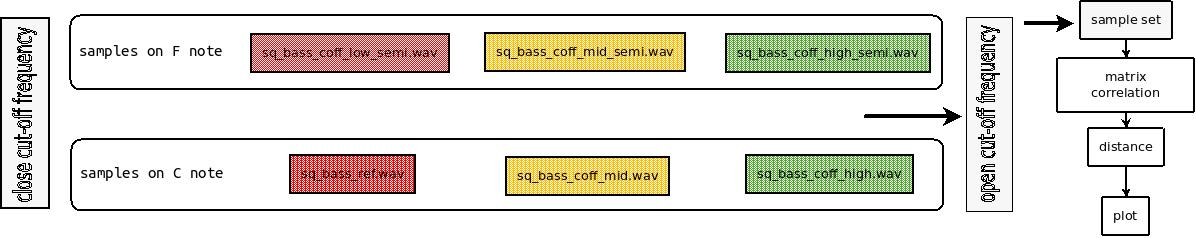
\includegraphics{/home/ion/Formacion/git_repo_klone/personal_projects/Master_thesis/TFM_iebs/Script/Diagram.jpeg}
\caption{image}
\end{figure}

\newpage

Six audio samples have been created from the same source and with the
following characteristics:

\begin{longtable}[]{@{}ll@{}}
\toprule
X\_pitch-11.wav* & Wave Object \\
\midrule
\endhead
Number of Samples: & 13020 \\
Duration (seconds): & 0.295 \\
Samplingrate (Hertz): & 44100 \\
Channels (Mono/Stereo): & Mono \\
PCM (integer format): & TRUE \\
Bit (8/16/24/32/64): & 16 \\
Peak Freq & 96Hz@ -13,6dB \\
& \\
\bottomrule
\end{longtable}

\begin{longtable}[]{@{}ll@{}}
\toprule
X\_pitch-11\_d.wav & Wave Object \\
\midrule
\endhead
Peak Freq & 90Hz@ -7,4dB \\
\bottomrule
\end{longtable}

\begin{longtable}[]{@{}ll@{}}
\toprule
X\_pitch-11\_dd.wav & Wave Object \\
\midrule
\endhead
Peak Freq & 80Hz@ -4,4dB \\
\bottomrule
\end{longtable}

\begin{longtable}[]{@{}ll@{}}
\toprule
X\_pitch-22\_d.wav & Wave Object \\
\midrule
\endhead
Peak Freq & 182Hz@ -15,13dB \\
\bottomrule
\end{longtable}

\begin{longtable}[]{@{}ll@{}}
\toprule
X\_pitch-11\_dd.wav & Wave Object \\
\midrule
\endhead
Peak Freq & 169Hz@ -8,7dB \\
\bottomrule
\end{longtable}

\begin{longtable}[]{@{}ll@{}}
\toprule
X\_pitch-11\_dd.wav & Wave Object \\
\midrule
\endhead
Peak Freq & 147Hz@ -5,2dB \\
\bottomrule
\end{longtable}

The duration of the samples is the same the reason is to avoid the
lengths of different samples altering the results of the frequency
analysis, to emphasize that the reason why the samples are so serious is
that in such a low-frequency range it allows adding higher frequencies
through the distortion effect.

The elements of our test set are two groups of samples that start from a
common origin. ``\textbf{X\_pitch-11.wav}'':

The first group of samples refers to those having the nomenclature
\textbf{X\_pitch-11\_xx} samples only modified at the harmonic level by
a distortion effect applied in \textbf{X\_pitch-11\_d} couples of times
in \textbf{X\_pitch-11\_dd} with the same distortion parameters.

The second group of samples is \textbf{X\_pitch-22\_xx} samples
previously modified the frequency to X\_pitch-11 and distorting the
sample sound with the same distortion parameters applied in the first
group.

With this set, it is intended to visualize the operation of our model
with special emphasis on the frequency relationship between the samples
with and without distortion.

\vspace{15pt}

\newpage

\hypertarget{codigo}{%
\subsection{Codigo}\label{codigo}}

\begin{Shaded}
\begin{Highlighting}[]
\FunctionTok{library}\NormalTok{(tuneR)}
\FunctionTok{library}\NormalTok{(knitr)}
\FunctionTok{library}\NormalTok{(NatureSounds)}
\FunctionTok{library}\NormalTok{(seewave)}
\FunctionTok{library}\NormalTok{(warbleR) }
\FunctionTok{library}\NormalTok{(igraph) }
\FunctionTok{library}\NormalTok{(imager) }
\end{Highlighting}
\end{Shaded}

\begin{Shaded}
\begin{Highlighting}[]
\FunctionTok{setwd}\NormalTok{(}\StringTok{"\textasciitilde{}/Formacion/git\_repo\_klone/personal\_projects/Master\_thesis/TFM\_iebs/Script"}\NormalTok{)}

\NormalTok{todas\_las\_muestras }\OtherTok{\textless{}{-}} \FunctionTok{selection\_table}\NormalTok{(}\AttributeTok{whole.recs =} \ConstantTok{TRUE}\NormalTok{, }\AttributeTok{extended =} \ConstantTok{TRUE}\NormalTok{)}
\end{Highlighting}
\end{Shaded}

\begin{verbatim}
checking selections (step 1 of 2):
Expected 'extended_selection_table' size is ~7MB (~0.00671 GB) 
 Do you want to proceed? (y/n): 

'extended_selection_table' was not created
\end{verbatim}

\begin{Shaded}
\begin{Highlighting}[]
\NormalTok{sample\_acoust\_param }\OtherTok{\textless{}{-}} \FunctionTok{na.omit}\NormalTok{(}\FunctionTok{specan}\NormalTok{(todas\_las\_muestras, }\AttributeTok{wl =} \DecValTok{512}\NormalTok{, }\AttributeTok{fsmooth =} \FloatTok{0.1}\NormalTok{, }
                                      \AttributeTok{threshold =} \DecValTok{10}\NormalTok{, }\AttributeTok{wn =} \StringTok{"hanning"}\NormalTok{,}
                                      \AttributeTok{flim =} \FunctionTok{c}\NormalTok{(}\DecValTok{0}\NormalTok{, }\DecValTok{22}\NormalTok{), }\AttributeTok{bp =} \FunctionTok{c}\NormalTok{(}\DecValTok{0}\NormalTok{,}\DecValTok{20}\NormalTok{), }
                                      \AttributeTok{fast.spec =} \ConstantTok{FALSE}\NormalTok{, }\AttributeTok{ovlp =} \DecValTok{50}\NormalTok{, }
                                      \AttributeTok{pal =}\NormalTok{ reverse.gray.colors}\FloatTok{.2}\NormalTok{,}
                                      \AttributeTok{widths =} \FunctionTok{c}\NormalTok{(}\DecValTok{2}\NormalTok{, }\DecValTok{1}\NormalTok{), }\AttributeTok{main =} \ConstantTok{NULL}\NormalTok{, }
                                      \AttributeTok{plot =} \ConstantTok{TRUE}\NormalTok{, }\AttributeTok{all.detec =} \ConstantTok{FALSE}\NormalTok{)) }
\end{Highlighting}
\end{Shaded}

\begin{Shaded}
\begin{Highlighting}[]
\NormalTok{xcor }\OtherTok{\textless{}{-}} \FunctionTok{xcorr}\NormalTok{(todas\_las\_muestras, }\AttributeTok{bp =} \FunctionTok{c}\NormalTok{(}\DecValTok{0}\NormalTok{, }\DecValTok{20}\NormalTok{), }\AttributeTok{wl =} \DecValTok{512}\NormalTok{, }\AttributeTok{ovlp =} \DecValTok{99}\NormalTok{, }\AttributeTok{path =} \ConstantTok{NULL}\NormalTok{,}
              \AttributeTok{type =} \StringTok{"mfcc"}\NormalTok{, }\AttributeTok{method=} \DecValTok{1}\NormalTok{, }\AttributeTok{na.rm =} \ConstantTok{TRUE}\NormalTok{)}
\end{Highlighting}
\end{Shaded}

\begin{verbatim}
creating spectrogram matrices (step 1 of 2):
running cross-correlation (step 2 of 2):
\end{verbatim}

\begin{Shaded}
\begin{Highlighting}[]
\NormalTok{distancia }\OtherTok{\textless{}{-}} \FunctionTok{dist}\NormalTok{(xcor, }\AttributeTok{method =} \StringTok{"euclidean"}\NormalTok{)}
\end{Highlighting}
\end{Shaded}

\begin{Shaded}
\begin{Highlighting}[]
\NormalTok{valores }\OtherTok{\textless{}{-}} \FunctionTok{cmdscale}\NormalTok{(distancia, }\AttributeTok{eig =}\NormalTok{ T)}
\end{Highlighting}
\end{Shaded}

\begin{Shaded}
\begin{Highlighting}[]
\NormalTok{old.par }\OtherTok{\textless{}{-}} \FunctionTok{par}\NormalTok{(}\AttributeTok{mfrow=}\FunctionTok{c}\NormalTok{(}\DecValTok{1}\NormalTok{, }\DecValTok{2}\NormalTok{))}

\CommentTok{\#plot(modelo, type = "p", xlab = "Coord 1", ylab = "Coord 2")}
\FunctionTok{plot}\NormalTok{(xcor, }\AttributeTok{type =} \StringTok{"p"}\NormalTok{, }\AttributeTok{xlab =} \StringTok{"Coord 1"}\NormalTok{, }\AttributeTok{ylab =} \StringTok{"Coord 2"}\NormalTok{)}
\FunctionTok{text}\NormalTok{(xcor[,}\DecValTok{1}\NormalTok{],xcor[,}\DecValTok{2}\NormalTok{], }\AttributeTok{labels =} \FunctionTok{rownames}\NormalTok{(xcor), }\AttributeTok{pos =} \DecValTok{2}\NormalTok{, }\AttributeTok{cex =} \FloatTok{0.8}\NormalTok{ )}
\FunctionTok{matplot}\NormalTok{(xcor, }\AttributeTok{lty =} \DecValTok{1}\NormalTok{)}

\FunctionTok{par}\NormalTok{(old.par)}
\end{Highlighting}
\end{Shaded}

\begin{Shaded}
\begin{Highlighting}[]
\FunctionTok{plot}\NormalTok{(sample\_acoust\_param}\SpecialCharTok{$}\NormalTok{dfrange)}
\FunctionTok{title}\NormalTok{(}\AttributeTok{main =} \StringTok{"frecuencia dominante"}\NormalTok{, }\AttributeTok{cex =} \FloatTok{1.5}\NormalTok{,}\AttributeTok{col =} \StringTok{"red"}\NormalTok{, }\AttributeTok{font =} \DecValTok{3}\NormalTok{)}
\end{Highlighting}
\end{Shaded}

\begin{Shaded}
\begin{Highlighting}[]
\NormalTok{old.par }\OtherTok{\textless{}{-}} \FunctionTok{par}\NormalTok{(}\AttributeTok{mfrow=}\FunctionTok{c}\NormalTok{(}\DecValTok{2}\NormalTok{, }\DecValTok{3}\NormalTok{))}

\FunctionTok{plot}\NormalTok{(sample\_acoust\_param}\SpecialCharTok{$}\NormalTok{meanfreq)}
\FunctionTok{title}\NormalTok{(}\AttributeTok{main =} \StringTok{"Frecuencia media"}\NormalTok{, }\AttributeTok{cex =} \FloatTok{1.5}\NormalTok{,}\AttributeTok{col =} \StringTok{"red"}\NormalTok{, }\AttributeTok{font =} \DecValTok{3}\NormalTok{)}

\FunctionTok{plot}\NormalTok{(sample\_acoust\_param}\SpecialCharTok{$}\NormalTok{sd)}
\FunctionTok{title}\NormalTok{(}\AttributeTok{main =} \StringTok{"desviación estandar"}\NormalTok{, }\AttributeTok{cex =} \FloatTok{1.5}\NormalTok{,}\AttributeTok{col =} \StringTok{"red"}\NormalTok{, }\AttributeTok{font =} \DecValTok{3}\NormalTok{)}

\FunctionTok{plot}\NormalTok{(sample\_acoust\_param}\SpecialCharTok{$}\NormalTok{skew)}
\FunctionTok{title}\NormalTok{(}\AttributeTok{main =} \StringTok{"asimetria"}\NormalTok{, }\AttributeTok{cex =} \FloatTok{1.5}\NormalTok{,}\AttributeTok{col =} \StringTok{"red"}\NormalTok{, }\AttributeTok{font =} \DecValTok{3}\NormalTok{)}

\FunctionTok{plot}\NormalTok{(sample\_acoust\_param}\SpecialCharTok{$}\NormalTok{kurt)}
\FunctionTok{title}\NormalTok{(}\AttributeTok{main =} \StringTok{"Pico del espectro"}\NormalTok{, }\AttributeTok{cex =} \FloatTok{1.5}\NormalTok{,}\AttributeTok{col =} \StringTok{"red"}\NormalTok{, }\AttributeTok{font =} \DecValTok{3}\NormalTok{)}

\FunctionTok{plot}\NormalTok{(sample\_acoust\_param}\SpecialCharTok{$}\NormalTok{sp.ent) }
\FunctionTok{title}\NormalTok{(}\AttributeTok{main =} \StringTok{"entropía espectral"}\NormalTok{, }\AttributeTok{cex =} \FloatTok{1.5}\NormalTok{,}\AttributeTok{col =} \StringTok{"red"}\NormalTok{, }\AttributeTok{font =} \DecValTok{3}\NormalTok{)}

\FunctionTok{plot}\NormalTok{(sample\_acoust\_param}\SpecialCharTok{$}\NormalTok{dfrange)}
\FunctionTok{title}\NormalTok{(}\AttributeTok{main =} \StringTok{"frecuencia dominante"}\NormalTok{, }\AttributeTok{cex =} \FloatTok{1.5}\NormalTok{,}\AttributeTok{col =} \StringTok{"red"}\NormalTok{, }\AttributeTok{font =} \DecValTok{3}\NormalTok{)}

\FunctionTok{par}\NormalTok{(old.par)}
\end{Highlighting}
\end{Shaded}

\begin{Shaded}
\begin{Highlighting}[]
\NormalTok{graf }\OtherTok{\textless{}{-}} \FunctionTok{graph.tree}\NormalTok{(}\FunctionTok{ncol}\NormalTok{(xcor),}\AttributeTok{mode =} \FunctionTok{c}\NormalTok{(}\StringTok{"in"}\NormalTok{))}
\FunctionTok{V}\NormalTok{(graf)}\SpecialCharTok{$}\NormalTok{label }\OtherTok{\textless{}{-}} \FunctionTok{colnames}\NormalTok{(xcor)}

\NormalTok{layout }\OtherTok{\textless{}{-}} \FunctionTok{layout.mds}\NormalTok{(graf, }\AttributeTok{dist =} \FunctionTok{as.matrix}\NormalTok{(distancia))}

\FunctionTok{plot}\NormalTok{(graf, }\AttributeTok{vertex.size =}\NormalTok{ .}\DecValTok{1}\NormalTok{)}
\end{Highlighting}
\end{Shaded}

\newpage

\hypertarget{muestras-y-anuxe1lisis}{%
\subsection{1 Muestras y análisis}\label{muestras-y-anuxe1lisis}}

Visualizamos las muestras cargadas en el espacio de trabajo

\begin{Shaded}
\begin{Highlighting}[]
\NormalTok{todas\_las\_muestras }
\end{Highlighting}
\end{Shaded}

\begin{verbatim}
Object of class 'selection_table' 
* The output of the following call: 
selection_table(whole.recs = TRUE, extended = TRUE) 

Contains: 
*  A selection table data frame with 6 rows and 5 columns: 
|sound.files                | selec| channel| start|    end|
|:--------------------------|-----:|-------:|-----:|------:|
|sq_bass_coff_high_semi.wav |     1|       1|     0| 6.4283|
|sq_bass_coff_high.wav      |     1|       1|     0| 6.4341|
|sq_bass_coff_low_semi.wav  |     1|       1|     0| 6.4647|
|sq_bass_coff_mid_semi.wav  |     1|       1|     0| 6.4479|
|sq_bass_coff_mid.wav       |     1|       1|     0| 6.4361|
|sq_bass_ref.wav            |     1|       1|     0| 6.4416|

 * A data frame (check.results) generated by check_sels() (as attribute) 
created by warbleR 1.1.27
\end{verbatim}

\newpage

\hypertarget{espectrogramas}{%
\subsection{1.1 Espectrogramas}\label{espectrogramas}}

Representación en tres dimensiones, temporal, frecuencial y amplitud de
la distribución de energía de una señal.

El espectrograma es el resultado de calcular la distribución de las
amplitudes para cada frecuencia de un fenómeno ondulatorio que sea lal
superposición de ondas de varias frecuencias de tramas de una señal. Una
gráfica tridimensional que representa la energía del contenido
frecuencial de la señal según va variando a lo largo del tiempo.

\begin{figure}
\centering
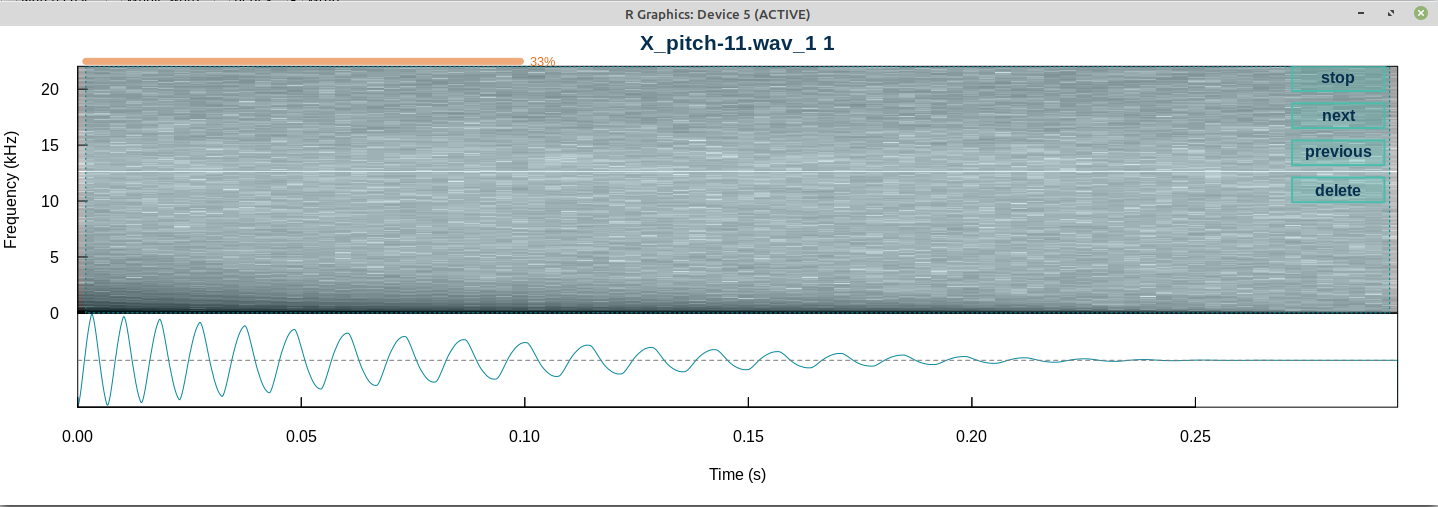
\includegraphics{/home/ion/Formacion/git_repo_klone/personal_projects/Master_thesis/TFM_iebs/Script/X_pitch-11.png}
\caption{X\_pitch-11.png}
\end{figure}

\vspace{15pt}

\begin{figure}
\centering
\includegraphics{/home/ion/Formacion/git_repo_klone/personal_projects/Master_thesis/TFM_iebs/ScriptX_pitch-11_d.png}
\caption{image}
\end{figure}

\vspace{15pt}

\begin{figure}
\centering
\includegraphics{/home/ion/Formacion/git_repo_klone/personal_projects/Master_thesis/TFM_iebs/ScriptX_pitch-11_dd.png}
\caption{image}
\end{figure}

\vspace{15pt}

\begin{figure}
\centering
\includegraphics{/home/ion/Formacion/git_repo_klone/personal_projects/Master_thesis/TFM_iebs/ScriptX_pitch-22.png}
\caption{image}
\end{figure}

\vspace{15pt}

\begin{figure}
\centering
\includegraphics{/home/ion/Formacion/git_repo_klone/personal_projects/Master_thesis/TFM_iebs/ScriptX_pitch-22_d.png}
\caption{image}
\end{figure}

\vspace{15pt}

\begin{figure}
\centering
\includegraphics{/home/ion/Formacion/git_repo_klone/personal_projects/Master_thesis/TFM_iebs/ScriptX_pitch-22_dd.png}
\caption{image}
\end{figure}

\newpage

\hypertarget{parametros-acusticos-de-las-muestras}{%
\subsection{1.2 Parametros acusticos de las
muestras}\label{parametros-acusticos-de-las-muestras}}

\begin{Shaded}
\begin{Highlighting}[]
\FunctionTok{head}\NormalTok{(sample\_acoust\_param,}\DecValTok{6}\NormalTok{)}
\end{Highlighting}
\end{Shaded}

\begin{verbatim}
                 sound.files selec duration  meanfreq       sd freq.median
1 sq_bass_coff_high_semi.wav     1 6.428299 1.4122415 2.021394   0.7011239
2      sq_bass_coff_high.wav     1 6.434150 1.3354086 1.996666   0.5871839
3  sq_bass_coff_low_semi.wav     1 6.464671 0.6865610 2.072786   0.3464998
4  sq_bass_coff_mid_semi.wav     1 6.447891 0.7183485 1.819615   0.3598099
5       sq_bass_coff_mid.wav     1 6.436122 0.6926713 1.752622   0.2694199
6            sq_bass_ref.wav     1 6.441587 0.6253070 2.056384   0.2656193
   freq.Q25  freq.Q75  freq.IQR time.median time.Q25 time.Q75 time.IQR     skew
1 0.3434838 1.7304865 1.3870027    2.518963 1.087866 3.705725 2.617859 41.87808
2 0.2656160 1.6034877 1.3378717    2.600420 1.111142 3.909357 2.798215 39.00662
3 0.1842327 0.3755810 0.1913483    2.001662 1.041563 3.258520 2.216957 53.88744
4 0.2728041 0.6822429 0.4094388    2.042608 1.012575 3.293778 2.281203 56.85685
5 0.2367912 0.5397721 0.3029809    2.316073 1.000916 3.334447 2.333531 53.43913
6 0.1966918 0.3421537 0.1454619    2.013360 1.012499 3.270255 2.257756 61.57953
      kurt    sp.ent  time.ent   entropy        sfm   meandom     mindom
1 3027.981 0.7831882 0.8851859 0.6932671 0.09223964 0.3240856 0.04306641
2 2406.148 0.7797894 0.8851991 0.6902689 0.09161440 0.2677277 0.04306641
3 4324.337 0.6920144 0.8852500 0.6126058 0.05771224 0.3058025 0.04306641
4 4524.267 0.7066747 0.8852144 0.6255586 0.04566056 0.3151962 0.04306641
5 4049.538 0.7081722 0.8851882 0.6268657 0.05711101 0.2445089 0.04306641
6 5295.176 0.6753334 0.8851988 0.5978043 0.06210927 0.2431227 0.04306641
     maxdom   dfrange   modindx  startdom     enddom     dfslope meanpeakf
1 0.5598633 0.5167969 17.666667 0.3875977 0.04306641 -0.05359602 0.3889541
2 5.4694336 5.4263672  3.476190 0.3014648 1.07666016  0.12048139 0.3024822
3 2.1102539 2.0671875  5.666667 0.3875977 0.04306641 -0.05329447 0.3889541
4 0.7321289 0.6890625 11.250000 0.5598633 0.04306641 -0.08014975 0.3889541
5 0.5598633 0.5167969 14.000000 0.3014648 0.30146484  0.00000000 0.3024822
6 0.3875977 0.3445312 18.750000 0.3014648 0.04306641 -0.04011409 0.3024822
\end{verbatim}

\textbf{duration}: longitud de la señal en segundos.

\vspace{6pt}

\textbf{meanfreq}: frecuencia media (en kHz). Media del espectro de
frecuencias (es decir, media ponderada de la frecuencia por la amplitud
dentro del paso de banda suministrado).

\vspace{6pt}

\textbf{sd}: Desviación estándar de la frecuencia (en kHz).

\vspace{6pt}

\textbf{freq.median}: frecuencia media. La frecuencia en la que la señal
se divide en dos intervalos de frecuencia de igual energía (en kHz).

\vspace{6pt}

\textbf{freq.Q25}: la primera frecuencia de cuartil. La frecuencia en la
que la señal se divide en dos intervalos de frecuencia de 25\% y 75\% de
energía respectivamente (en kHz).

\vspace{6pt}

\textbf{freq.Q75}: frecuencia del tercer cuartil. La frecuencia en la
que la señal se divide en dos intervalos de frecuencia de 75\% y 25\% de
energía respectivamente (en kHz).

\vspace{6pt}

\textbf{freq.IQR}: rango de frecuencia intercuartil. Gama de frecuencias
entre `freq.Q25' y `freq.Q75' (en kHz).

\vspace{6pt}

\textbf{time.median}: tiempo medio. El tiempo en el que la señal se
divide entre dos intervalos.

\vspace{6pt}

\textbf{time.Q25}: el primer tiempo de cuartil. El tiempo en el que la
señal se divide en dos intervalos de tiempo de 25\% y 75\% de energía
respectivamente (en s).

\vspace{6pt}

\textbf{time.Q75}: el tiempo del tercer cuartil. El tiempo en el que la
señal se divide en dos intervalos de tiempo de 75\% y 25\% de energía
respectivamente (en s).

\vspace{6pt}

\textbf{time.IQR}: rango de tiempo intercuartílico. Rango de tiempo
entre ``tiempo.Q25'' y ``tiempo.Q75'' (en s).

\vspace{6pt}

\textbf{skew}: asimetría. Asimetría del espectro.

\vspace{6pt}

\textbf{kurt}: Picos del espectro

\vspace{6pt}

\textbf{sp.ent}: Distribución energética del espectro de frecuencias.
Tono puro \textasciitilde{} 0; ruidoso \textasciitilde{} 1.

\vspace{6pt}

\textbf{time.ent}: entropía del tiempo. Distribución de la energía en la
envoltura del tiempo. Tono puro \textasciitilde{} 0; ruidoso
\textasciitilde{} 1.

\vspace{6pt}

\textbf{entropy}: entropía espectrográfica. Producto del tiempo y la
entropía espectral \textbf{sp.ent * time.ent}.

\vspace{6pt}

\textbf{sfm}: planitud espectral. Similar a sp.ent (Tono puro
\textasciitilde{} 0; ruidoso \textasciitilde{} 1).

\vspace{6pt}

\textbf{meandom}: promedio de la frecuencia dominante medida a través de
la señal acústica.

\vspace{6pt}

\textbf{mindom}: mínimo de la frecuencia dominante medida a través de la
señal acústica.

\vspace{6pt}

\textbf{maxdom}: máximo de la frecuencia dominante medida a través de la
señal acústica.

\vspace{6pt}

\textbf{dfrange}: rango de frecuencia dominante medido a través de la
señal acústica.

\vspace{6pt}

\textbf{modindx}: índice de modulación. Calculado como la diferencia
absoluta acumulada entre las mediciones adyacentes de las frecuencias
dominantes dividida por la gama de frecuencias dominantes. 1 significa
que la señal no está modulada , 0 que sí lo está.

\vspace{6pt}

\textbf{startdom}: medición de la frecuencia dominante al inicio de la
señal.

\vspace{6pt}

\textbf{enddom}: medición de la frecuencia dominante al final de la
señal.

\vspace{6pt}

\textbf{dfslope}: pendiente del cambio de la frecuencia dominante a
través del tiempo ((enddom-startdom)/duración). Las unidades son kHz/s.

\vspace{6pt}

\textbf{meanpeakf}: frecuencia media de pico. Frecuencia con la mayor
energía del espectro de frecuencia media.

\vspace{6pt}

\hypertarget{definir-el-modelo}{%
\subsection{2 Definir el modelo:}\label{definir-el-modelo}}

En el procesamiento de señales, la correlación cruzada (o a veces
denominada ``covarianza cruzada'') es una medida de la similitud entre
dos señales, frecuentemente usada para encontrar características
relevantes en una señal desconocida por medio de la comparación con otra
que sí se conoce. Es una función del tiempo relativa a las señales, a
veces también se la llama producto escalar desplazado, y tiene
aplicaciones en el reconocimiento de patrones y en criptoanálisis de las
muestras sonoras por medio de la correlación cruzada tiempo-frecuencia.

Primero se crean las matrices (manteniéndolas internamente como una
lista) y se calcula la correlación cruzada en un segundo paso.

El cepstrum de frecuencia de mel (MFC) es una representación del
espectro de potencia a corto plazo de un sonido, basado en una
transformación coseno lineal de un espectro de potencia logarítmica en
una escala de frecuencia de mel no lineal. \newpage

\hypertarget{matriz-de-similitud}{%
\subsection{2.1 Matriz de similitud}\label{matriz-de-similitud}}

\begin{Shaded}
\begin{Highlighting}[]
\NormalTok{xcor }
\end{Highlighting}
\end{Shaded}

\begin{verbatim}
                             sq_bass_coff_high_semi.wav-1
sq_bass_coff_high_semi.wav-1                    1.0000000
sq_bass_coff_high.wav-1                         0.6604942
sq_bass_coff_low_semi.wav-1                     0.2494178
sq_bass_coff_mid_semi.wav-1                     0.3177522
sq_bass_coff_mid.wav-1                          0.1627039
sq_bass_ref.wav-1                               0.1334896
                             sq_bass_coff_high.wav-1
sq_bass_coff_high_semi.wav-1               0.6604942
sq_bass_coff_high.wav-1                    1.0000000
sq_bass_coff_low_semi.wav-1                0.1428839
sq_bass_coff_mid_semi.wav-1                0.1426412
sq_bass_coff_mid.wav-1                     0.3387273
sq_bass_ref.wav-1                          0.2642610
                             sq_bass_coff_low_semi.wav-1
sq_bass_coff_high_semi.wav-1                   0.2494178
sq_bass_coff_high.wav-1                        0.1428839
sq_bass_coff_low_semi.wav-1                    1.0000000
sq_bass_coff_mid_semi.wav-1                    0.7795262
sq_bass_coff_mid.wav-1                         0.4808978
sq_bass_ref.wav-1                              0.4426888
                             sq_bass_coff_mid_semi.wav-1 sq_bass_coff_mid.wav-1
sq_bass_coff_high_semi.wav-1                   0.3177522              0.1627039
sq_bass_coff_high.wav-1                        0.1426412              0.3387273
sq_bass_coff_low_semi.wav-1                    0.7795262              0.4808978
sq_bass_coff_mid_semi.wav-1                    1.0000000              0.4637285
sq_bass_coff_mid.wav-1                         0.4637285              1.0000000
sq_bass_ref.wav-1                              0.3695036              0.8441879
                             sq_bass_ref.wav-1
sq_bass_coff_high_semi.wav-1         0.1334896
sq_bass_coff_high.wav-1              0.2642610
sq_bass_coff_low_semi.wav-1          0.4426888
sq_bass_coff_mid_semi.wav-1          0.3695036
sq_bass_coff_mid.wav-1               0.8441879
sq_bass_ref.wav-1                    1.0000000
\end{verbatim}

\hypertarget{calculo-de-las-distancias}{%
\subsection{2.3 Calculo de las
distancias}\label{calculo-de-las-distancias}}

Medida de distancia especificada para calcular las distancias entre las
filas de una matriz de datos.

\begin{Shaded}
\begin{Highlighting}[]
\NormalTok{distancia}
\end{Highlighting}
\end{Shaded}

\begin{verbatim}
                            sq_bass_coff_high_semi.wav-1
sq_bass_coff_high.wav-1                        0.5662395
sq_bass_coff_low_semi.wav-1                    1.3434115
sq_bass_coff_mid_semi.wav-1                    1.2753153
sq_bass_coff_mid.wav-1                         1.4441772
sq_bass_ref.wav-1                              1.4707596
                            sq_bass_coff_high.wav-1 sq_bass_coff_low_semi.wav-1
sq_bass_coff_high.wav-1                                                        
sq_bass_coff_low_semi.wav-1               1.4477401                            
sq_bass_coff_mid_semi.wav-1               1.4211316                   0.3279297
sq_bass_coff_mid.wav-1                    1.2946134                   0.9196402
sq_bass_ref.wav-1                         1.3255932                   0.9744033
                            sq_bass_coff_mid_semi.wav-1 sq_bass_coff_mid.wav-1
sq_bass_coff_high.wav-1                                                       
sq_bass_coff_low_semi.wav-1                                                   
sq_bass_coff_mid_semi.wav-1                                                   
sq_bass_coff_mid.wav-1                        0.9757911                       
sq_bass_ref.wav-1                             1.0497640              0.2555225
\end{verbatim}

\hypertarget{escalado-multidimensional}{%
\subsection{2.3 Escalado
multidimensional}\label{escalado-multidimensional}}

Escalamiento multidimensional (MDS) de una matriz de datos. También
conocido como análisis de coordenadas principales.

\begin{Shaded}
\begin{Highlighting}[]
\NormalTok{valores\_distancia }\OtherTok{\textless{}{-}} \FunctionTok{as.data.frame}\NormalTok{(valores}\SpecialCharTok{$}\NormalTok{points)}
\end{Highlighting}
\end{Shaded}

\newpage

\hypertarget{evaluar-el-modelo}{%
\subsection{3 Evaluar el modelo}\label{evaluar-el-modelo}}

\hypertarget{visualizacion}{%
\subsection{3.1 Visualizacion}\label{visualizacion}}

En esta primera representación vemos la disposición de los elementos de
nuestro conjunto en un espacio bidimensional indicando cual es la
similitud frecuencial que existe entre las muestras.

Representación de los valores de la matriz de correlación

\includegraphics{TFM_iebs_eng_files/figure-latex/3.1 Visualizacion en un sistema de coordenadas -1.pdf}

Únicos elementos (V1 y V2) que reprentan al conjunto de muestras tras
haber sido analizado.

\newpage

\hypertarget{conclusiones}{%
\subsection{CONCLUSIONES}\label{conclusiones}}

El objetivo inicial de visualizar las diferencias frecuencial entre los
elementos de un conjunto mediante el escalamiento multidimensional ha
sido llevado a buen término.

El analisis de la relación frecuencial a partir del conjunto de muestras
nos ha dotado de un dataset de datos unico.

Se ha observado que dado que el ejercicio es muy sencillo y no incluye
elementos que tengan en cuenta la duración de las muestras, es necesario
que las muestras tengan la misma duración ya que es muy importante a la
hora de hacer la correlación frecuencial cruzada y no interferir en el
resultado.

\vspace{45pt}

\includegraphics{TFM_iebs_eng_files/figure-latex/09b PLOT-3-1.pdf}

\includegraphics{TFM_iebs_eng_files/figure-latex/3.1 Visualizacion en un sistema de coordenadas xcorr-1.pdf}
Esta es la representación gráfica de los elementos de la matríz de
correlación

Las muestras a las que no se les a doblado la frequencia
\textbf{X\_pitch-11.wav, X\_pitch-11\_d.wav, X\_pitch-11\_dd.wav} en la
parte inferior izquierda y aquellas a las que si se les ha modificado la
frecuencia \textbf{X\_pitch-22.wav X\_pitch-22\_d.wav
X\_pitch-22\_dd.wav} y se encuentran mas a la derecha del gráfico.

Cabe destacar que ambos grupos de muestras comparten el mismo indice de
distorsión en las muestras y que debido a ello se puede verse claramente
reflejado en el eje de coordenadas 2.

\includegraphics{TFM_iebs_eng_files/figure-latex/07b PLOT-2 -1.pdf}

Cada una de las columnas de la matríz de correlación es comparada contra
las demás columnas de la matriz, cada columna representa una muestra de
sonido.

Se aprecia que la distorsión máxima que se le ha aplicado a las muestras
influyen en el resultado a nivel frecuencial, esto se puede observar en
la 2 columna y en la 5, ya que es donde mayor diferencia (son las más
distorsionadas) entre las muestras del mismo grupo.

Conforme más arriba en la columna esté la muestra que comparamos más
parecido tendrá ese sonido con la muestra comparada.

Se observa que existe una mayor similitud entre la muestra 1
X\_pitch-11\_d.wav (columna) y las muestras X\_pitch-11\_dd.wav (2) y
X\_pitch-11.wav (3) que entre X\_pitch-11\_d.wav (1) y las muestras
X\_pitch-22\_d.wav (4), X\_pitch-22\_dd.wav (5) y X\_pitch-22.wav (6).

\includegraphics{TFM_iebs_eng_files/figure-latex/08b PLOT-2 colorines-1.pdf}

Observamos dos grupos claramente diferenciados gracias al análisis de
las coordenadas principales (PCA).

\newpage

\hypertarget{resultados}{%
\subsection{RESULTADOS}\label{resultados}}

Para evaluar el modelo le pasaré una libreria de sonido de 8 bits que
hice hace un tiempo y que contiene 172 elementos.

\begin{Shaded}
\begin{Highlighting}[]
\FunctionTok{library}\NormalTok{(ggplot2)}
\FunctionTok{library}\NormalTok{(ggfortify)}

\NormalTok{  alles\_dir }\OtherTok{\textless{}{-}} \StringTok{"/home/ion/Formacion/00\_iebs/TFM\_iebs/TFM\_iebs/Data/8bits"}

\NormalTok{wav\_names }\OtherTok{\textless{}{-}} \FunctionTok{list.files}\NormalTok{(alles\_dir, }\AttributeTok{pattern =} \StringTok{"}\SpecialCharTok{\textbackslash{}\textbackslash{}}\StringTok{.wav$"}\NormalTok{)}

\NormalTok{sound\_design }\OtherTok{\textless{}{-}} \FunctionTok{selection\_table}\NormalTok{(}\AttributeTok{whole.recs =} \ConstantTok{TRUE}\NormalTok{, }\AttributeTok{path =}\NormalTok{ alles\_dir, }\AttributeTok{extended =} \ConstantTok{TRUE}\NormalTok{)}
\end{Highlighting}
\end{Shaded}

\begin{verbatim}
checking selections (step 1 of 2):
Expected 'extended_selection_table' size is ~23MB (~0.02228 GB) 
 Do you want to proceed? (y/n): 

'extended_selection_table' was not created
\end{verbatim}

\begin{Shaded}
\begin{Highlighting}[]
\NormalTok{xcor }\OtherTok{\textless{}{-}} \FunctionTok{xcorr}\NormalTok{(sound\_design, }\AttributeTok{bp =} \FunctionTok{c}\NormalTok{(}\DecValTok{0}\NormalTok{, }\DecValTok{20}\NormalTok{), }\AttributeTok{wl =} \DecValTok{512}\NormalTok{, }\AttributeTok{ovlp =} \DecValTok{99}\NormalTok{, }\AttributeTok{path =}\NormalTok{ alles\_dir,}
              \AttributeTok{type =} \StringTok{"mfcc"}\NormalTok{, }\AttributeTok{method=} \DecValTok{1}\NormalTok{, }\AttributeTok{na.rm =} \ConstantTok{TRUE}\NormalTok{,}
              \AttributeTok{parallel =} \DecValTok{4}\NormalTok{)}
\end{Highlighting}
\end{Shaded}

\begin{verbatim}
creating spectrogram matrices (step 1 of 2):
running cross-correlation (step 2 of 2):
\end{verbatim}

\begin{Shaded}
\begin{Highlighting}[]
\NormalTok{distancia }\OtherTok{\textless{}{-}} \FunctionTok{dist}\NormalTok{(xcor, }\AttributeTok{method =} \StringTok{"euclidean"}\NormalTok{)}
  
\NormalTok{valores }\OtherTok{\textless{}{-}} \FunctionTok{cmdscale}\NormalTok{(distancia, }\AttributeTok{eig =}\NormalTok{ T)}



\FunctionTok{autoplot}\NormalTok{(}\FunctionTok{cmdscale}\NormalTok{(distancia, }\AttributeTok{eig =}\NormalTok{ T), }\AttributeTok{label =} \ConstantTok{TRUE}\NormalTok{, }\AttributeTok{label.size =} \DecValTok{3}\NormalTok{, }\AttributeTok{frame =} \ConstantTok{TRUE}\NormalTok{)}
\end{Highlighting}
\end{Shaded}

\includegraphics{TFM_iebs_eng_files/figure-latex/sound_design 01-1.pdf}

Vemos que hay muestras que estan mas ``juntas'', estas son aquellas que
tienen una mayor similitud frecuencial entre ellas. Llegados a este
punto dariamos por concluida la busqueda de una herramienta que nos
permitiera saber cual es la predominancia frecuencial de nuestra
libreria de sonidos.

\vspace{15pt}

\newpage

\hypertarget{referencias}{%
\subsection{REFERENCIAS}\label{referencias}}

\vspace{15pt}

Araya-Salas, M. and Smith-Vidaurre, G. (2017), warbleR: an r package to
streamline analysis of animal acoustic signals. Methods Ecol Evol. 8,
184-191.

Maechler, M., Rousseeuw, P., Struyf, A., Hubert, M., Hornik, K.(2019).
cluster: Cluster Analysis Basics and Extensions. R package version 2.1.0

NOTE: please also cite the `tuneR' and `seewave' packages if you use any
spectrogram-creating or acoustic-measuring function

Uwe Ligges, Sebastian Krey, Olaf Mersmann, and Sarah Schnackenberg
(2018). tuneR: Analysis of Music and Speech. URL:
\url{https://CRAN.R-project.org/package=tuneR}

Yihui Xie (2020). knitr: A General-Purpose Package for Dynamic Report
Generation in R. R package version 1.30.

Yihui Xie (2015) Dynamic Documents with R and knitr. 2nd edition.
Chapman and Hall/CRC. ISBN 978-1498716963

Yihui Xie (2014) knitr: A Comprehensive Tool for Reproducible Research
in R. In Victoria Stodden, Friedrich Leisch and Roger D. Peng, editors,
Implementing Reproducible Computational Research. Chapman and Hall/CRC.
ISBN 978-1466561595

Araya-Salas, M. (2018), \emph{NatureSounds: a collection of animal sound
for bioacoustic analysis in the R environment}. R package version 1.1.0.

Sueur J, Aubin T, Simonis C (2008). seewave: a free modular tool for
sound analysis and synthesis. Bioacoustics, 18: 213-226

Araya-Salas, M. and Smith-Vidaurre, G. (2017), warbleR: an r package to
streamline analysis of animal acoustic signals. Methods Ecol Evol. 8,
184-191.

\end{document}
